\appendix

\chapter{Numerical simulation with \texttt{axionbloch}}\label{app:axionbloch}
\begin{jointwork}
    This appendix is adapted from Ref.\,\cite{Zhang2026_axionbloch}.
\end{jointwork}

Analytical estimates of the ALP-induced spin-precession signal (Chapter~\ref{chap:theory}) are valid in the long-dwell-time limit $T \gg \tau_a,\,T_2^*,\,T_2$.
At lower Compton frequencies, the ALP coherence time becomes comparable to or longer than experimentally accessible dwell times, and the scaling laws no longer apply.
Numerical simulation is then the tool of choice.
This appendix describes \texttt{axionbloch}, an open-source Python package that simulates spin dynamics under both magnetic and axion-induced pseudomagnetic fields.


% \section{Spin dynamics: the Bloch equations}\label{sec:axionbloch:bloch}

% The package models spin-$1/2$ ensembles through the Bloch equations~\eqref{eq:bloch_x}--\eqref{eq:bloch_z} derived in Section~\ref{sec:intro:bloch_eq}. The total effective field is $\mathbf{B}_\mathrm{eff} = \mathbf{B}_0 + \mathbf{B}_a(t)$, combining the laboratory bias field and the axion-induced pseudomagnetic field. The equations are solved in the rotating coordinate frame (RCF), which removes the fast Larmor precession and exposes the slow axion-induced dynamics. The effective transverse relaxation time $T_2^*$ (which includes inhomogeneous broadening) is simulated by sampling the spread of bias-field values from a \texttt{Magnet} instance and integrating the Bloch equations for each sampled field independently.


% \section{Numerical integration}\label{sec:axionbloch:rk4}

% The time evolution of $\mathbf{M}$ is obtained by numerically integrating Equations~(\ref{eq:bloch_x}--\ref{eq:bloch_z}) with the fourth-order Runge--Kutta (RK4) method. Given a time step $\Delta t$ and initial magnetization $\mathbf{M}^n$, the update rule is
% \begin{equation}
%     \mathbf{M}^{n+1}
%     = \mathbf{M}^n
%     + \frac{\Delta t}{6}\bigl(\mathbf{k}_1 + 2\mathbf{k}_2 + 2\mathbf{k}_3 + \mathbf{k}_4\bigr)\,,
% \end{equation}
% where $\mathbf{k}_1 = d\mathbf{M}/dt|_{\mathbf{M}^n}$ and subsequent $\mathbf{k}_i$ are evaluated at intermediate half-steps following the standard RK4 prescription. The local truncation error is $\mathcal{O}(\Delta t^5)$ and the global accumulated error is $\mathcal{O}(\Delta t^4)$. The time step is set to be at least one order of magnitude smaller than the shortest characteristic timescale in the simulation (e.g., $T_1$, $T_2$, or $1/\nu_a$).

% The RK4 integration is implemented in a compiled C++ backend and exposed to Python through the \texttt{pybind11} interface, achieving runtimes of $\sim\SI{10}{\s}$ for $\approx4\times10^9$ integration steps on a modern desktop CPU.


\section{Software architecture}\label{sec:axionbloch:arch}

The package uses an object-oriented design separating three concerns: experimental configuration (\texttt{Sample}, \texttt{Magnet}), field generation (\texttt{MagField}), and simulation management (\texttt{Simulation}, \texttt{Simulations}).
Axion-field models are encapsulated in dedicated classes (e.g., \texttt{MilkyWayAxionHalo}), allowing new models to be added without modifying the simulation framework.
The architecture is illustrated in Figure~\ref{fig:axionbloch_arch}.

\begin{figure}[htb]
    \centering
    \fbox{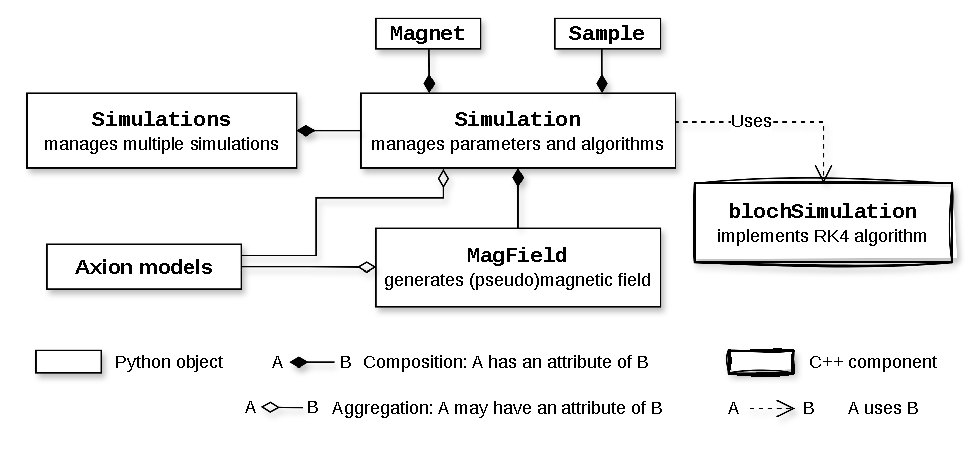
\includegraphics[width=0.95\linewidth]{figures/AxionBloch_diagram.drawio.pdf}}
    \caption{Architecture of \texttt{axionbloch}.
    Each \texttt{Simulation} instance receives parameters from \texttt{Magnet}, \texttt{Sample}, and \texttt{MagField}.
    For axion simulations, an axion-model object is required both to configure the simulation and to generate the pseudomagnetic field.
    Numerical integration is performed via the \texttt{blochSimulation} API, which provides Python access to the C++ backend.
    Reproduced from Ref.\,\cite{Zhang2026_axionbloch}.}
    \label{fig:axionbloch_arch}
\end{figure}


\section{Calibration}\label{sec:axionbloch:calibration}

Three standard NMR experiments are used to benchmark the simulation against known analytical results.

\subsection{Pulsed NMR: free decay and spin echo}

After a $\SI{90}{\degree}$ pulse, the magnetization tips into the transverse plane and decays with the dephasing time $T_2^*$ (free decay).
A subsequent $\SI{180}{\degree}$ pulse refocuses the inhomogeneous dephasing, producing a spin echo whose amplitude decays with the true $T_2$.
The simulated signals reproduce both behaviors, calibrating the pulse-induced rotation, Larmor precession, and transverse relaxations.
The simulated magnetization is shown in Figure~\ref{fig:calibration_NMR}\,(a).

\subsection{Continuous-wave NMR}

For a weak oscillating field on resonance ($\gamma B T_2^* \ll 1$), the transverse magnetization grows as $\gamma B T_2^*(1 - e^{-t/T_2^*})$\,\cite{Abragam1961_NuclearMagnetism}.
The simulation reproduces this analytical form, as shown in Figure~\ref{fig:calibration_NMR}\,(b).
This benchmark calibrates both the Larmor precession and the $T_2^*$ relaxation under continuous driving---the same physical regime as the ALP-induced signal.

\begin{figure}[htb]
    \centering
    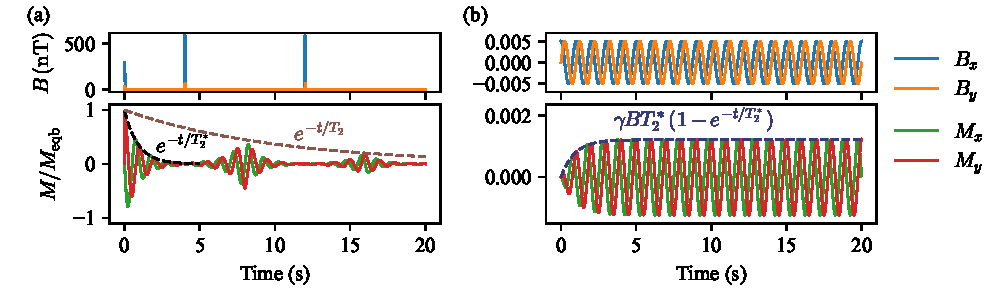
\includegraphics[width=\linewidth]{figures/SpinEcho_and_CW.pdf}
    \caption{Calibration of \texttt{axionbloch} against analytical NMR results.
    Upper rows: applied transverse magnetic fields; lower rows: normalized simulated magnetization.
    \textbf{(a)} After $\SI{90}{\degree}$ and $\SI{180}{\degree}$ pulses, the simulation produces free decay (timescale $T_2^*$) and a spin echo (timescale $T_2$).
    \textbf{(b)} Under a weak continuous-wave drive on resonance, the transverse magnetization grows as $\gamma B T_2^*(1-e^{-t/T_2^*})$ (dashed line).
    Reproduced from Ref.\,\cite{Zhang2026_axionbloch}.}
    \label{fig:calibration_NMR}
\end{figure}

\subsection{Hyperpolarized sample and $T_1$ relaxation}

Hyperpolarization boosts the initial spin polarization above its thermal value.
In the simulation, the initial polarization is set as a parameter of the \texttt{Sample} class.
A sample polarized significantly above thermal equilibrium relaxes toward $M_\mathrm{eqb}$ with the longitudinal time constant $T_1$.
The simulated $M_z(t) = M_\mathrm{eqb}[1-(M_\mathrm{eqb}^\mathrm{init}/M_\mathrm{eqb} - 1)e^{-t/T_1}]$ reproduces the expected exponential approach to equilibrium, as illustrated in Figure~\ref{fig:calibration_T1}.

\begin{figure}[htb]
    \centering
    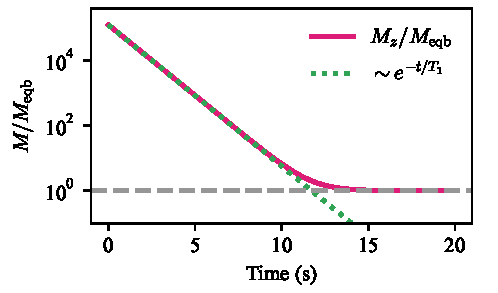
\includegraphics[width=0.75\linewidth]{figures/T1_hyperpolarized.pdf}
    \caption{Simulated $T_1$ relaxation of a hyperpolarized sample in a static bias field.
    The axial magnetization $M_z$ is normalized by the equilibrium magnetization $M_\mathrm{eqb}$.
    The exponential approach to equilibrium calibrates the longitudinal relaxation in the simulation.
    Reproduced from Ref.\,\cite{Zhang2026_axionbloch}.}
    \label{fig:calibration_T1}
\end{figure}


\section{Axion simulation example}\label{sec:axionbloch:example}

As a demonstration, the \texttt{MilkyWayAxionHalo} model simulates the pseudomagnetic field from virialized galactic dark matter following the standard halo model\,\cite{Evans2019_SHMRefined,Gramolin2022Feb_SpectralSignatures}.
The axion field oscillates at the Compton frequency with a Maxwell-Boltzmann velocity distribution setting the spectral linewidth.
The stochasticity of the field amplitude is accounted for by generating many independent realizations of the pseudomagnetic field.

Figure~\ref{fig:axion_sim} shows results for a \ch{^{129}Xe} sample polarized to \SI{50}{\%}.
A single realisation (left) illustrates the stochastic fluctuations in both the pseudomagnetic field and the induced transverse magnetization.
An ensemble of 1000 realizations (right) yields the mean signal and its standard deviation band.
The signal initially grows as the ALP field drives the magnetization away from equilibrium, and then decays on the $T_1$ timescale as the hyperpolarization is lost.

These simulations validate the three-regime picture \YZ{add reference to the analytical three-regime expression}: at low frequencies where $\tau_a \gg T$, the signal grows linearly in dwell time; in the intermediate regime $\tau_a \sim T$, the signal departs from the analytical long-dwell-time scaling; and at high frequencies where $T \gg \tau_a$, the analytical results apply directly.

\begin{figure}[htb]
    \centering
    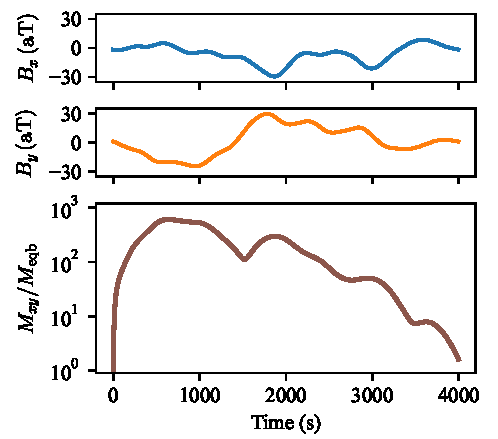
\includegraphics[width=0.49\linewidth]{figures/MilkyWayAxionHalo-1.pdf}
    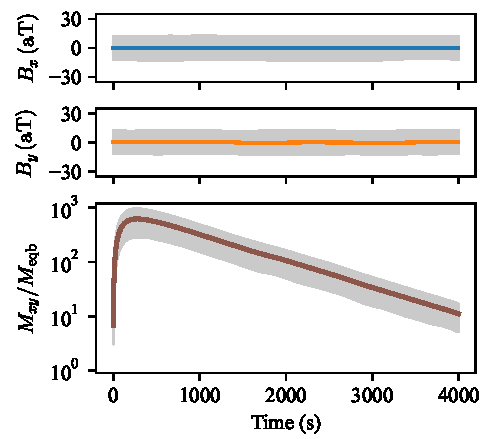
\includegraphics[width=0.49\linewidth]{figures/MilkyWayAxionHalo-1000.pdf}
    \caption{Simulated axion-induced NMR signals for a virialized Milky Way axion dark matter halo.
    Upper panels: pseudomagnetic fields $B_x$ and $B_y$ in the transverse plane.
    Lower panels: amplitude of the induced transverse magnetization $M_{xy}$, normalized by $M_\mathrm{eqb}$.
    Left: single simulation realisation.
    Right: ensemble of 1000 realizations; solid lines show the mean and shaded bands show $\pm\sigma$.
    The sample is \ch{^{129}Xe} initially polarized to \SI{50}{\%}.
    Reproduced from Ref.\,\cite{Zhang2026_axionbloch}.}
    \label{fig:axion_sim}
\end{figure}


\section{Statistical hypothesis test for ALP detection}\label{app:hypothesis}

\section{The Neyman--Pearson Lemma}

The \emph{Neyman--Pearson lemma} is a foundational result in statistical hypothesis testing.
It establishes the form of the most powerful test for discriminating between two simple hypotheses at a fixed significance level.

\subsection{Problem setup}

Suppose we observe data $x$ drawn from a probability distribution.
We wish to test
\[
H_0 : x \sim f_0(x)
\]
against
\[
H_1 : x \sim f_1(x),
\]
where both $f_0(x)$ and $f_1(x)$ are fully specified probability density functions.
The goal is to construct a test that maintains a fixed false-alarm probability (Type~I error) while maximizing the probability of correctly detecting the alternative hypothesis (power).

\subsection{Likelihood ratio and the lemma}

The key quantity is the likelihood ratio
\[
\Lambda(x) = \frac{f_1(x)}{f_0(x)}.
\]
For a fixed significance level $\alpha$, the Neyman--Pearson lemma states that the most powerful test rejects $H_0$ when $\Lambda(x) > k$, where $k$ satisfies $P(\Lambda(x)>k\mid H_0)=\alpha$.
The likelihood-ratio test is therefore optimal among all tests with the same false-positive rate.

\subsection{Type I error and power}

The significance level $\alpha = P(\text{reject }H_0\mid H_0\text{ true})$ is the false-alarm probability.
The power $1-\beta = P(\text{reject }H_0\mid H_1\text{ true})$ is the probability of correctly detecting an ALP signal.
The Neyman--Pearson lemma guarantees that the likelihood-ratio test maximizes the power for fixed $\alpha$.

\subsection{Application to the ALP search}

In the ALP data analysis described in Section~\ref{sec:results:data-analysis}, the normalized power excess (NPE) plays the role of the test statistic.
The null hypothesis is that a $5\,\sigma$ ALP signal is present; the alternative is that no signal is present.
Monte Carlo simulations of the NPE distribution under the null hypothesis determine the threshold $\Theta_\mathrm{RE} = 3.43$ corresponding to the \SI{95}{\%} confidence level (see Section~\ref{sec:results:data-analysis}).

\subsection{Gaussian example}

For $X\sim\mathcal{N}(\mu,\sigma^2)$ with $H_0:\mu=0$ versus $H_1:\mu=1$, the log-likelihood ratio simplifies to $\log\Lambda(x) = x/\sigma^2 - 1/(2\sigma^2)$, so rejecting for large $\Lambda(x)$ is equivalent to rejecting for large $x$.
This confirms that the sample mean is the optimal test statistic for Gaussian location testing.

\section{Optimal filter as a weighted average}\label{sec:app:optimal-filter}

The optimal filter used in the ALP search can be understood as the linear combination of frequency bins that maximizes the signal-to-noise ratio.
Consider a baseline-subtracted spectrum with bin values $x_i$ near a trial ALP frequency.
If the expected ALP lineshape in these bins is $s_i$, the signal model can be written as
\begin{equation}
    x_i = A s_i + n_i\,,
\end{equation}
where $A$ is the signal amplitude and $n_i$ is noise.
The noise in a power spectrum follows a $\chi^2$ distribution with two degrees of freedom before averaging.
After subtracting the local mean, the noise fluctuations have zero mean but are not Gaussian.
The following result therefore states optimality among linear filters, rather than optimality among all possible statistical tests.

For a general linear statistic $T=\sum_i w_i x_i$, the signal-to-noise ratio is
\begin{equation}
    \mathrm{SNR}(T)
    =
    \frac{A\sum_i w_i s_i}
         {\left(\sum_{ij} w_i C_{ij} w_j\right)^{1/2}}\,,
\end{equation}
where $C_{ij}=\langle n_i n_j\rangle$ is the noise covariance matrix.
Maximizing this expression gives
\begin{equation}
    \mathbf{w}\propto \mathbf{C}^{-1}\mathbf{s}\,.
    \label{eq:optimal_filter_covariance}
\end{equation}
If the frequency bins are independent, $C_{ij}=\sigma_i^2\delta_{ij}$, and the optimal linear estimator combines the bins as
\begin{equation}
    \hat{A} =
    \frac{\sum_i s_i x_i/\sigma_i^2}
         {\sum_i s_i^2/\sigma_i^2}\,.
    \label{eq:optimal_filter_estimator}
\end{equation}
Equivalently, the filtered spectrum is a weighted average of the neighboring bins, with weights proportional to $s_i/\sigma_i^2$.
If the noise variance is approximately constant across the linewidth, the weights are proportional to the expected ALP lineshape.
Thus the optimal linear filter is matched to the expected ALP lineshape and reduces to a lineshape-weighted average when the local noise level is uniform.


\section{Optimal dwell time in frequency scanning}\label{app:dwell_time}
% \begin{jointwork}
%     This appendix is adapted from Ref.\,\cite{Yuzhe2023_FrequencyScanning}.
% \end{jointwork}

This appendix derives the optimal dwell-time allocation scheme for a frequency scan, following the treatment of Ref.\,\cite{Yuzhe2023_FrequencyScanning}.
The goal is to maximize the sensitive area in the $\log\nu$--$\log|g_{\mathrm{aNN}}|$ parameter space over a total measurement time $T_{\mathrm{tot}}$.

To simplify the notation, the frequency is normalized: $\hat{\nu} = \nu/\nu_{\mathrm{start}}$, with $\hat{\nu} \in [1,\,\hat{\nu}_{\mathrm{end}}]$ where $\hat{\nu}_{\mathrm{end}} = \nu_{\mathrm{end}}/\nu_{\mathrm{start}} > 1$.
The dwell time is parameterized as
\begin{equation}
    T = \kappa\,\hat{\nu}^{\,n}
    \,,\label{eq:T_kappa_n}
\end{equation}
where $\kappa$ is determined by $T_{\mathrm{tot}}$ and $n$, and the optimal value of $n$ is determined below.

\subsection{Regimes (1)--(3): step size proportional to $\nu$}

In regimes~(1), (2), and~(3), the frequency-step size is proportional to $\hat{\nu}$ (either one ALP linewidth $\hat{\nu}/Q_a$ or one NMR linewidth $\delta_\nu\hat{\nu}$).
The scan rate is
\begin{equation}
    \dfrac{d\hat{\nu}}{dt} = \dfrac{\Gamma_{\mathrm{scan}}}{T} \propto \hat{\nu}^{1-n}
    \,,
\end{equation}
so that
\begin{equation}
    dt = \kappa\,C\,\hat{\nu}^{n-1}\,d\hat{\nu}
    \,,
\end{equation}
where $C = Q_a$ in regime~(1) and $C = \delta_\nu^{-1}$ in regimes~(2) and~(3).
Integrating over $[0,\,T_{\mathrm{tot}}]$ and $[1,\,\hat{\nu}_{\mathrm{end}}]$ gives
\begin{equation}
    \kappa = \dfrac{n\,T_{\mathrm{tot}}}{C(\hat{\nu}_{\mathrm{end}}^{n}-1)}
    \,,\quad n \ne 0\,.
\end{equation}
At $n=0$: $\kappa|_{n=0} = T_{\mathrm{tot}}/[C\ln(\hat{\nu}_{\mathrm{end}})]$.

\subsection{Regime (4): step size independent of $\nu$}

In regime~(4) ($T_2^*=T_2 \ll \tau_a$), the step size is one NMR linewidth $2/T_2$, independent of frequency.
The scan rate is proportional to $\hat{\nu}^{-n}$, giving
\begin{equation}
    \kappa = \dfrac{2(n+1)\,T_{\mathrm{tot}}}{(\hat{\nu}_{\mathrm{end}}^{n+1}-1)\,T_2}
    \,,\quad n \ne -1\,.
\end{equation}
At $n=-1$: $\kappa|_{n=-1} = 2T_{\mathrm{tot}}/[\ln(\hat{\nu}_{\mathrm{end}})\,T_2]$.

\subsection{Optimal exponent $n$}

The sensitive area in log-log scale is
\begin{equation}
    A(n) = -\int_{1}^{\hat{\nu}_{\mathrm{end}}} \log f(\hat{\nu},\,n)\,d\log\hat{\nu}
    \,,\label{eq:A_n}
\end{equation}
where $f(\hat{\nu},\,n)$ is the exclusion threshold from Equation~\eqref{eq:exclusion_threshold} with the dwell time from Equation~\eqref{eq:T_kappa_n}.
Taking the derivative $A'(n)$ and setting it to zero shows:
\begin{itemize}
    \item For regimes~(1), (2), and~(3): $A'(n) > 0$ for $n < 0$ and $A'(n) < 0$ for $n > 0$, so the maximum is at $n = 0$ (uniform dwell time).
    \item For regime~(4): the analysis shifts the effective exponent from $n$ to $n+1$, giving an optimum at $n = -1$ (dwell time $T \propto \hat{\nu}^{-1}$).
\end{itemize}

An intuitive restatement: when the sensitive bandwidth per step grows with frequency (regimes 1--3), the number of steps per unit $\log\nu$ is constant, and uniform dwell time is optimal.
When the bandwidth is independent of frequency (regime 4), spending less time at higher frequencies---where the ALP coherence time is shorter and the signal integrates faster---maximizes the covered area.

\section{ALP candidate lists}\label{app:candidates}


The outliers appeared in at least two independent scan steps with consistent frequencies and coupling strengths are regarded as ALP candidates. 
This appendix lists the ALP candidates identified in the Milky Way and Earth-halo searches.
% The candidate tables are ordered as MW first and EH second, matching the discussion in Chapter~\ref{chap:results}.
% \subsection{Milky Way ALP candidates}

\begin{table}[htb]
    \centering
    \caption{Milky Way ALP candidates.}
    \label{tab:mw_candidates}
    \begin{tabular}{cccc}
        \hline\hline
        Index & Step index & Frequency (\unit{\Hz}) & Mass (\unit{\neV/c^2}) \\
        \hline
        1 & 5, 27 & 1348668.58 & 5.57764506\\
        2 & 66, 86, 102 & 1348485.70 & 5.57688873\\
        3 & 111, 117, 128 & 1348792.89 & 5.57815918\\
        4 & 126, 140 & 1348872.72 & 5.57848936\\
        5 & 7, 10 & 1348686.37 & 5.57771866\\
        6 & 29, 95 & 1348769.02 & 5.57806045\\
        \hline\hline
    \end{tabular}
\end{table}

% \subsection{Earth-halo ALP candidates}

\begin{longtable}{cccc}
    \caption{Earth-halo ALP candidates.}
    \label{tab:eh_candidates}\\
    \hline\hline
    Index & Step index & Frequency (\unit{\Hz}) & Mass (\unit{\neV/c^2}) \\
    \hline
    \endfirsthead

    \hline\hline
    Index & Step index & Frequency (\unit{\Hz}) & Mass (\unit{\neV/c^2}) \\
    \hline
    \endhead

    \hline\hline
    \endfoot

    \hline\hline
    \endlastfoot

    1 & 7 & 1348672.0739 & 5.5776595297\\
    2 & 2 & 1348646.2182 & 5.5775525993\\
    3 & 7 & 1348646.2294 & 5.5775526455\\
    4 & 7 & 1348646.2375 & 5.5775526792\\
    5 & 7 & 1348646.2472 & 5.5775527189\\
    6 & 3 & 1348514.7177 & 5.5770087568\\
    7 & 4 & 1348505.8949 & 5.5769722685\\
    8 & 5 & 1348505.3398 & 5.5769699730\\
    9 & 5 & 1348505.3520 & 5.5769700234\\
    10 & 5 & 1348505.8094 & 5.5769719150\\
    11 & 5 & 1348505.8120 & 5.5769719257\\
    12 & 5 & 1348505.8628 & 5.5769721358\\
    13 & 5 & 1348505.9028 & 5.5769723014\\
    14 & 5 & 1348505.9126 & 5.5769723419\\
    15 & 5 & 1348505.9161 & 5.5769723564\\
    16 & 5 & 1348595.9240 & 5.5773445990\\
    17 & 5 & 1348595.9522 & 5.5773447157\\
    18 & 5 & 1348595.9537 & 5.5773447217\\
    19 & 5 & 1348595.9770 & 5.5773448182\\
    20 & 5 & 1348595.9908 & 5.5773448753\\
    21 & 5 & 1348596.0179 & 5.5773449876\\
    22 & 5 & 1348596.0282 & 5.5773450299\\
    23 & 5 & 1348646.2350 & 5.5775526685\\
    24 & 5 & 1348646.2589 & 5.5775527675\\
    25 & 6 & 1348505.8143 & 5.5769719353\\
    26 & 6 & 1348505.8432 & 5.5769720548\\
    27 & 6 & 1348505.8699 & 5.5769721653\\
    28 & 6 & 1348505.8731 & 5.5769721784\\
    29 & 6 & 1348505.8740 & 5.5769721821\\
    30 & 6 & 1348505.8809 & 5.5769722106\\
    31 & 6 & 1348505.8885 & 5.5769722423\\
    32 & 6 & 1348505.8896 & 5.5769722469\\
    33 & 6 & 1348505.8963 & 5.5769722745\\
    34 & 6 & 1348595.9210 & 5.5773445867\\
    35 & 6 & 1348595.9736 & 5.5773448042\\
    36 & 6 & 1348596.0053 & 5.5773449353\\
    37 & 6 & 1348596.0214 & 5.5773450017\\
    38 & 6 & 1348596.0231 & 5.5773450090\\
\end{longtable}
